\section{Syntax and Semantics}

\begin{frame}[fragile]
\frametitle{What is a program?}

A program is a sequence of one of more statements written to perform a task in a computer:

\begin{example}
\begin{semiverbatim}
x = 21;
y = 21;
z = x + y;
\end{semiverbatim}
\end{example}


\end{frame}

\subsection{Expressions}

\begin{frame}[fragile]
\frametitle{Syntax of expressions}
\framesubtitle{Expressions in Chloe}

\begin{columns}[t]
\column{.45\textwidth}
\begin{semiverbatim}
\textbf{type_synonym} \textit{vname} = string

\textbf{datatype} \textit{exp} = Const \textit{int}
  | Null
  | V      \textit{vname}
  | Plus  \textit{exp} \textit{exp}
  | Subst \textit{exp} \textit{exp}
  | Minus \textit{exp}
  | Div   \textit{exp} \textit{exp}
  | Mod   \textit{exp} \textit{exp}
  | Mult  \textit{exp} \textit{exp}
  | Less  \textit{exp} \textit{exp}
  | Not   \textit{exp}
\end{semiverbatim}
\column{.45\textwidth}
\begin{semiverbatim}
  | And   \textit{exp} \textit{exp}
  | Or    \textit{exp} \textit{exp}
  | Eq    \textit{exp} \textit{exp}
  | New   \textit{exp}
  | Deref \textit{exp}
  | Ref   \textit{lexp}
  | Index \textit{exp} \textit{exp}
and
\textbf{datatype} \textit{lexp} = Deref \textit{exp}
  | Indexl \textit{exp} \textit{exp}
\end{semiverbatim}
\end{columns}


\end{frame}


\begin{frame}[fragile]
\frametitle{Syntax of expressions}
\framesubtitle{Expressions in Chloe}

Why do we have \textit{exp} and \textit{lexp}?
\begin{example}
\begin{semiverbatim}
foo = *bar;
*baz = 1;
\end{semiverbatim}
\end{example}



\end{frame}


\begin{frame}[fragile]
\frametitle{Types}
\framesubtitle{Integers}

Integers are 64 bit length words.
\begin{block}{}
\begin{semiverbatim}
\textbf{type_synonym} int_width = 64
\textbf{type_synonym} int_val = int_width word
\end{semiverbatim}
\end{block}
They have the following bounds:
\begin{block}{}
\begin{semiverbatim}
INT_MIN == - (2^(int_width - 1))
INT_MAX ==  ((2^(int_width - 1)) - 1)
\end{semiverbatim}
\end{block}

\end{frame}

\begin{frame}
\frametitle{Types}
\framesubtitle{Addresses}

An address is a pair representing a block id and an offset.

\begin{semiverbatim}
\textbf{datatype} addr = nat $\times$ int
\end{semiverbatim}

\end{frame}

\begin{frame}[fragile]
\frametitle{Values}
\framesubtitle{}

\begin{semiverbatim}
\textbf{datatype} val = NullVal
             | I \textit{int_val}
             | V \textit{vname}
\end{semiverbatim}

\end{frame}

\begin{frame}[fragile]
\frametitle{Dynamic memory}
\framesubtitle{Layout of the heap}

\begin{semiverbatim}
\textbf{type_synonym} mem = val option list option list
\end{semiverbatim}


\begin{columns}[t]
\column{.45\textwidth}
\begin{block}{Example memory layout}
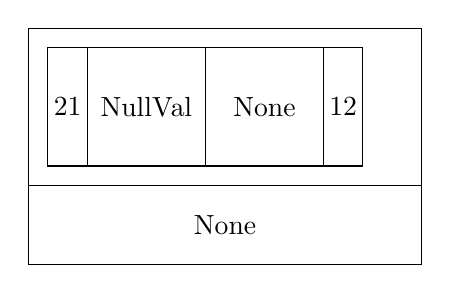
\begin{tikzpicture}
\alert<2>{\draw (0,0) rectangle (5,2);}
\alert<3>{\draw (0,-1) rectangle (5,0) node[midway] {None};}
\alert<4>{\draw (0.25,0.25) rectangle (0.75,1.75) node[midway] {21};}
\draw (0.75,0.25) rectangle (2.25,1.75) node[midway] {NullVal};
\alert<5>{\draw (2.25,0.25) rectangle (3.75,1.75) node[midway] {None};}
\draw (3.75,0.25) rectangle (4.25,1.75) node[midway] {12};
\end{tikzpicture}
\end{block}
\column{.45\textwidth}
\begin{itemize}
\alert<2>{\item{Allocated block}}
\alert<3>{\item{Unallocated block}}
\alert<4>{\item{Initialized cell}}
\alert<5>{\item{Uninitialized cell}}
\end{itemize}
\end{columns}


\end{frame}


\begin{frame}[fragile]
\frametitle{Dynamic Memory}
\framesubtitle{Memory management operations}

\begin{itemize}
\item<1-3>{new\_block :: $val\ \Rightarrow\ mem\ \Rightarrow\ (val\ \times\ mem)$ option}
\item<1,2,4>{free :: $addr\ \Rightarrow\ val\ \Rightarrow\ visible\_state\ \Rightarrow\ visible\_state$ option}
\item<1,2,5>{load :: $addr\ \Rightarrow\ mem\ \Rightarrow\ val$ option}
\item<1,2,6>{store :: $addr\ \Rightarrow\ val\ \Rightarrow\ visible\_state\ \Rightarrow\ visible\_state$ option}
\end{itemize}

\alert<2>{Return types are $\tau$ option, these functions can always fail}

\end{frame}


\begin{frame}[fragile]
\frametitle{Unlimited memory problem}
\framesubtitle{Possible solutions}

Our memory allocation cannot fail because we assume unlimited memory.

\bigskip

However, we have limited resources in a machine.

There are two possible solutions:

\begin{itemize}
\item{Model non-deterministic behavior in our \verb|new_block| function.}
\item{Assume a fixed amount of memory.}
\end{itemize}


\end{frame}


\begin{frame}
\frametitle{Unlimited memory problem}
\framesubtitle{Our solution}

We keep our unlimited memory assumption.

\bigskip
Later in the translation process we wrap C's malloc function in one of our own.

\bigskip
This function checks if a malloc call fails.

\bigskip
If it fails, then the program will be aborted.


\end{frame}


\begin{frame}
\frametitle{Semantics of expressions}
\framesubtitle{What is the meaning of an expression?}

The semantics of an expression is its value and effect on the program state.

\pause
\begin{example}
$21 + 21 = 42$

\pause

$foo + 42 = ?$

\pause

$bar = new (12)$
\end{example}
\pause

We need to know the value of a variable at the time of execution.



\end{frame}


\begin{frame}[fragile]
\frametitle{Semantics of expressions}
\framesubtitle{Valuations}

A valuation is a function that maps a variable name to a value.

\bigskip
\pause

\textbf{type\_synonym} valuation = vname $\Rightarrow$ val option option

\bigskip

\pause
Given a variable name it can yield three results:

\bigskip

\pause
\begin{itemize}
\item{None: undefined variable.}
\pause
\item{Some None: uninitialized variable.}
\pause
\item{Some $v$: initializeid variable holding value $v$.}
\end{itemize}


\end{frame}


\begin{frame}
\frametitle{Semantics of expressions}
\framesubtitle{Visible state}

When we execute a command it can only \textit{see} certain part of the state:

\bigskip
\pause

\textbf{type\_synonym} visible\_state = valuation $\times$ valuation $\times$ mem

\bigskip
\pause
\begin{itemize}
\item{Local variables to the current function}
\pause
\item{Global variables}
\pause
\item{Memory}
\end{itemize}


\end{frame}


\begin{frame}
\frametitle{Semantics of expressions}
\framesubtitle{Evaluation functions eval and eval\_l}

We define functions to compute the values of an expressions:

\bigskip

\textbf{eval} :: exp $\Rightarrow$ visible\_state $\Rightarrow$ (val $\times$ visible\_state) option

\textbf{eval\_l} :: exp $\Rightarrow$ visible\_state $\Rightarrow$ (addr $\times$ visible\_state) option

\bigskip

The evaluation of functions can fail:

\bigskip
\pause

\begin{itemize}
\item{Undefined variables}
\pause
\item{Illegal operands given to the function}
\pause
\item{Trying to access invalid memory}
\pause
\item{Integer overflow}
\pause
\item{Division by zero}
\end{itemize}


\end{frame}


\begin{frame}
\frametitle{Semantics of expressions}
\framesubtitle{Highlights of expression evaluation}

\begin{itemize}
\item{Integer overflow is detected and leads to an erroneous state}
\item{Short-circuit evaluation}
\item{Division and modulo towards zero}
\item{Static scoping of variables}
\end{itemize}


\end{frame}


\subsection{Commands}


\begin{frame}[fragile]
\frametitle{Syntax of commands}
\framesubtitle{Concrete syntax}

\begin{semiverbatim}
com ::= SKIP
     | lexp ::== exp
     | vname ::= exp
     | com ;; com
     | IF exp THEN com ELSE com
     | WHILE exp DO com
     | FREE lexp
     | RETURN exp
     | RETURNV
     | lexp ::== f ( [exp] )
     | vname ::= f ( [exp] )
     | CALL f ( [exp])
\end{semiverbatim}


\end{frame}


\begin{frame}[fragile]
\frametitle{Syntax of commands}
\framesubtitle{Abstract syntax}

\begin{semiverbatim}
\textbf{datatype} com = SKIP
             | Assignl lexp exp
             | Assign  vname exp
             | Seq     com  com
             | If      exp com com
             | While   exp com
             | Free    lexp
             | Return exp
             | Returnv
             | Callfunl lexp fname " exp list"
             | Callfun vname fname " exp list"
             | Callfunv fname " exp list"
\end{semiverbatim}

\end{frame}


\begin{frame}[fragile]
\frametitle{Functions}
\framesubtitle{}

We have functions that return a value and those that do not.

\begin{semiverbatim}
\textbf{record} fun_decl =
  name :: fname
  params :: vname list
  locals :: vname list
  body :: com
\end{semiverbatim}

\bigskip

A function is valid $\Longleftrightarrow$ the function parameters and the local variables have different names

\bigskip

When a function returns a value, this value will be:

\begin{itemize}
\item{Assigned to a location in memory}
\item{Assigned to a variable}
\item{Ignored}
\end{itemize}


\end{frame}


\begin{frame}[fragile]
\frametitle{Programs}

\begin{semiverbatim}
\textbf{record} program =
  name :: fname
  globals :: vname list
  procs :: fun_decl list
\end{semiverbatim}
\pause

\begin{block}{A program is considered valid if:}
\begin{itemize}
\item{The global variable names are different from one another.}
\pause
\item{Function names within a program are different from one another.}
\pause
\item{All function declarations are valid.}
\pause
\item{The main function is defined.}
\pause
\item{None of the variable names or function names in the program is a reserved keyword.}
\pause
\item{Global variables and function names are disjoint.}
\end{itemize}
\end{block}


\end{frame}


\begin{frame}[fragile]
\frametitle{Stack}
\framesubtitle{Return locations and stack frames}

\begin{semiverbatim}
\textbf{datatype} return_loc = \alert<3>{Ar \textit{addr}} | \alert<4>{Vr \textit{vname}} | \alert<5>{Invalid}
\end{semiverbatim}

\pause

A return value of a function can be:
\begin{itemize}
\item<3->{\alert<3>{Assigned to a cell in memory}}
\item<4->{\alert<4>{Assigned to a variable}}
\item<5->{\alert<5>{Ingnored}}
\end{itemize}


\bigskip
\onslide<6->{\textbf{datatype} stack\_frame = com $\times$ valuation $\times$ return\_loc}

\bigskip

\onslide<6>{The execution stack is a list of stack frames.}


\end{frame}


\begin{frame}
\frametitle{Stack}
\framesubtitle{Calling convention}


\end{frame}


\begin{frame}
\frametitle{Procedure table}
\framesubtitle{}


\end{frame}


\begin{frame}
\frametitle{State}
\framesubtitle{Components of a state}


\end{frame}


\begin{frame}
\frametitle{State}
\framesubtitle{Initial state}


\end{frame}


\begin{frame}
\frametitle{State}
\framesubtitle{Why do we need an initial state?}


\end{frame}


\subsection{Small-step semantics}


\begin{frame}
\frametitle{Control Flow Graph}
\framesubtitle{What is a CFG?}


\end{frame}


\begin{frame}
\frametitle{Control Flow Graph}
\framesubtitle{Enabled functions}


\end{frame}


\begin{frame}
\frametitle{Control Flow Graph}
\framesubtitle{Enabled functions: if-then-else example}


\end{frame}


\begin{frame}
\frametitle{Control Flow Graph}
\framesubtitle{Transformer functions: why do we need them?}


\end{frame}


\begin{frame}
\frametitle{Control Flow Graph}
\framesubtitle{How do our transformer functions behave?}


\end{frame}


\begin{frame}
\frametitle{Control Flow Graph}
\framesubtitle{... with a stack}


\end{frame}


\begin{frame}
\frametitle{Control Flow Graph}
\framesubtitle{Rules}


\end{frame}


\begin{frame}
\frametitle{Small-step semantics}
\framesubtitle{Rules}


\end{frame}


\begin{frame}
\frametitle{Small-step semantics}
\framesubtitle{When can a step be taken?}


\end{frame}


\begin{frame}
\frametitle{Small-step semantics}
\framesubtitle{When does taking a step fail?}


\end{frame}


\begin{frame}
\frametitle{Small-step semantics}
\framesubtitle{How do we take several steps?}


\end{frame}


\subsection{Interpreter}

\begin{frame}
\frametitle{Interpreter}
\framesubtitle{Taking a single step}


\end{frame}


\begin{frame}
\frametitle{Interpreter}
\framesubtitle{Final states}


\end{frame}


\begin{frame}
\frametitle{Interpreter}
\framesubtitle{Execution of a program}


\end{frame}
